\documentclass{article}
\usepackage[utf8]{inputenc}
\usepackage{vmargin}


\usepackage{amsmath} 
\usepackage{graphicx}
\usepackage{graphics}
\usepackage{float}
\usepackage{blindtext}
\usepackage{listings}
\usepackage{xcolor}
\usepackage[spanish]{babel}
\usepackage{subfig}

\graphicspath{ {images/} }
\title{Operador Logarítmico}
\date{}
\setpapersize{A4}
\setmargins{2.5cm}       % margen izquierdo
{1.5cm}                        % margen superior
{16.5cm}                      % anchura del texto
{23.42cm}                    % altura del texto
{10pt}                           % altura de los encabezados
{1cm}                           % espacio entre el texto y los encabezados
{0pt}                             % altura del pie de página
{2cm}                           % espacio entre el texto y el pie de página

\begin{document}

%-------COLORES PARA CODIGO ------------------------
\lstdefinestyle{customc}{
  belowcaptionskip=1\baselineskip,
  breaklines=true,
  frame=L,
  xleftmargin=\parindent,
  language=JavaScript,
   basicstyle=\footnotesize\ttfamily,
  showstringspaces=false,
  basicstyle=\footnotesize\ttfamily,
  keywordstyle=\bfseries\color{green!40!black},
  commentstyle=\itshape\color{purple!40!black},
  identifierstyle=\color{blue},
  stringstyle=\color{orange},
  frame=single,	  
  numbers=left,
   numberstyle=\footnotesize,
}

\lstdefinestyle{customasm}{
  belowcaptionskip=1\baselineskip,
  frame=L,
  xleftmargin=\parindent,
  language=JavaScript,
  basicstyle=\footnotesize\ttfamily,
  commentstyle=\itshape\color{purple!40!black},
}

\lstset{escapechar=@,style=customc}

%---------------------------------------------

\thispagestyle{empty}

\vfill
 \begin{center}
    \begin{figure}[h]
    \centering
    \includegraphics[width=12cm]{unsa}\\
    
    \end{figure}
 	 
     \vspace*{1.5cm}
    {\large\bfseries FACULTAD DE PRODUCCIÓN Y SERVICIOS} \\
    {\large\bfseries ESCUELA PROFESIONAL DE CIENCIA DE LA COMPUTACIÓN}  \\    
    \vspace*{1.5cm}
    
 	\rule[0.5ex]{\linewidth}{2pt}\vspace*{-\baselineskip}\vspace*		{3.2pt}
	\rule[0.5ex]{\linewidth}{1pt}\\[\baselineskip]
 	{\huge Física Computacional} \\[4mm]
    \rule[0.5ex]{\linewidth}{1pt}\vspace*{-							\baselineskip}\vspace{3.2pt}
	\rule[0.5ex]{\linewidth}{2pt}\\
 	\vspace*{1cm}

    \begin{large} \bfseries
    Tarea Ley de la gravitación \\
    
    \vspace{5mm}
    Eduardo Antonio Sánchez Hincho \\

    \vspace{5mm}
    Docente:\\
    Edwin Agapito Llamoca Requena
    \end{large}
    \vspace*{0.4in}
    
    \noindent \\
    
    \vfill
    \large\bfseries{ AREQUIPA\\2020}
\end{center}
\newpage

\section{Movimiento de un proyectil}
\subsection{}
\begin{lstlisting}[language=Python,caption=1\_1.py]
h = 0.01
tiempo = 400
R = 2

pt = np.arange(0,tiempo,h)
lvx = np.arange(0,1,0.05)

ax = []
ay = []
vx = []
vy = []

cuerpo = plt.Circle((0, 0), R,lw=1,alpha=0.5)
plt.gcf().gca().add_artist(cuerpo)

for vx0 in lvx:
    x = 0
    y = 7
    vx = [vx0]
    vy = [0]
    px = [0,x]
    py = [0,y]
    for t in pt:
        ax.append(-x / (x**2 + y**2) ** (1.5))
        ay.append(-y / (x**2 + y**2) ** (1.5))
        vx.append(vx[-1] + ax[-1] * h)
        vy.append(vy[-1] + ay[-1] * h)
        x = x + vx[-1] * h
        y = y + vy[-1] * h
        if x >= 20:
            break
        if x**2 + y**2 <= R**2:
            break
        px.append(x)
        py.append(y)

    plt.plot(px,py)
plt.show()

\end{lstlisting}
\begin{figure}[H]
    \centering
    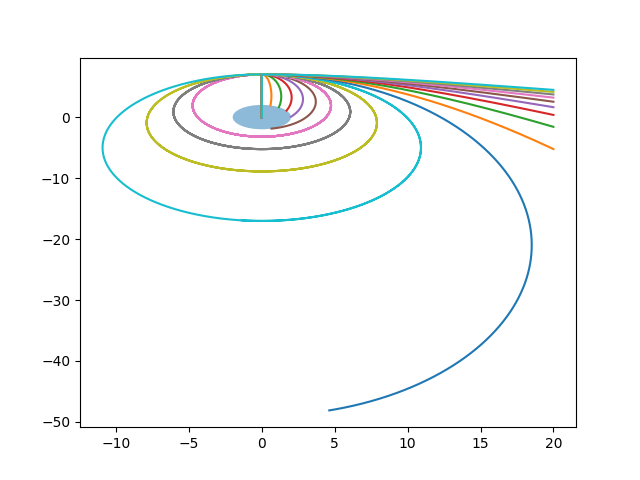
\includegraphics[width=0.5\textwidth]{1_1.png}
    \caption{Resultado}
\end{figure}

\subsection{}
\begin{lstlisting}[language=Python,caption=1\_2.py]
h = 0.01
tiempo = 10000
R = 1

pt = np.arange(0,tiempo,h)
lvx = np.arange(0,1,0.05)

ax = []
ay = []
vx = []
vy = []

cuerpo = plt.Circle((0, 0), R,lw=1,alpha=0.5)
plt.gcf().gca().add_artist(cuerpo)

for vx0 in lvx:
    x = 3
    y = 4
    vx = [vx0]
    vy = [0]
    px = [0,x]
    py = [0,y]
    for t in pt:
        ax.append(-x / (x**2 + y**2) ** (1.5))
        ay.append(-y / (x**2 + y**2) ** (1.5))
        vx.append(vx[-1] + ax[-1] * h)
        vy.append(vy[-1] + ay[-1] * h)
        x = x + vx[-1] * h
        y = y + vy[-1] * h
        if x >= 20:
            break
        if x**2 + y**2 <= R**2:
            break
        px.append(x)
        py.append(y)

    plt.plot(px,py)
plt.show()
\end{lstlisting}
\begin{figure}[H]
    \centering
    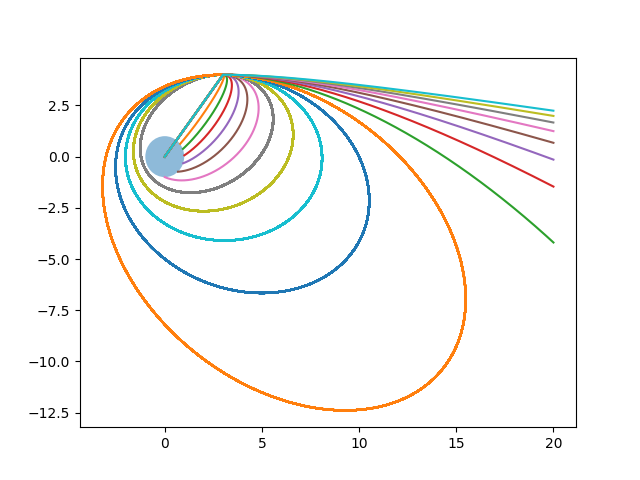
\includegraphics[width=0.5\textwidth]{1_2.png}
    \caption{Resultado}
\end{figure}

\section{Problema de 3 cuerpos}
\begin{lstlisting}[language=Python,caption=2.py]
h=0.01
t=1800

R=2
d=10

pt=np.arange(0,t,h)
lvx = np.arange(0,1,0.05)

ax = []
ay = []

cuerpo1 = plt.Circle((-d, 0), R,lw=1,alpha=0.5)
cuerpo2 = plt.Circle((d, 0),R,lw=1,alpha=0.5)

plt.gcf().gca().add_artist(cuerpo1)
plt.gcf().gca().add_artist(cuerpo2)

plt.xlim([-50,50])
plt.ylim([-50,50])

for vx0 in lvx:
    x=10
    y=10
    vx=vx0
    vy=0
    px=[x]
    py=[y]

    for t in pt:
        x1 = x + d
        x2 = x - d

        ax.append(-x1 / (x1**2 + y**2)**(1.5) - x2 / (x2**2 + y**2) ** 1.5)
        ay.append(-y / (x1**2+y**2)**(1.5) - y / (x2**2 + y**2) ** 1.5)
        
        vx = vx + ax[-1]*h;
        vy = vy + ay[-1]*h
        
        x = x + vx*h 
        y = y + vy*h
        
        if x >= 50:
            break
        if y >= 50:
            break
        if x1**2 + y**2 <= R**2:
            break
        if x2**2 + y**2 <= R**2:
            break
        px.append(x)
        py.append(y)

    plt.plot(px,py)

plt.show()
\end{lstlisting}
\begin{figure}[H]
    \centering
    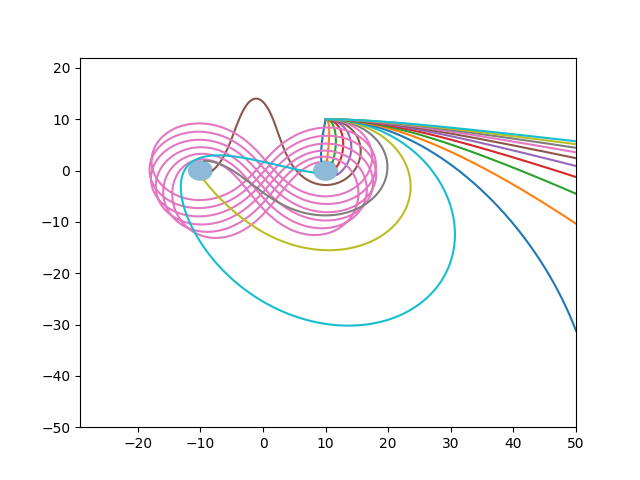
\includegraphics[width=0.5\textwidth]{2.png}
    \caption{Resultado}
\end{figure}

\section{Desafío 1}
\begin{lstlisting}[language=Python,caption=desafio.py]
h=0.01
t=10000

R=5
d=20
d2=20

pt=np.arange(0,t,h)
lvx = np.arange(0,1,0.05)

ax = []
ay = []

cuerpo1 = plt.Circle((-d, 0), R,lw=1,alpha=0.4)
cuerpo2 = plt.Circle((d, 0),R,lw=1,alpha=0.4)
cuerpo3 = plt.Circle((0, d2), R,lw=1,alpha=0.4)

plt.gcf().gca().add_artist(cuerpo1)
plt.gcf().gca().add_artist(cuerpo2)
plt.gcf().gca().add_artist(cuerpo3)

plt.xlim([-70,70])
plt.ylim([-70,70])

for vx0 in lvx:
    x = 15
    y = 40
    vx = vx0
    vy = 0
    px = [x]
    py = [y]

    for t in pt:
        x1 = x+d
        x2 = x-d
        x3 = x
        y2 = y-d2
        
        ax.append(-x1 / (x1**2 + y**2)**(1.5) - (x2 / (x2**2 + y**2)**(1.5)) - x3/ (x3**2 + y2**2)**(1.5))
        ay.append(-y / (x1**2 + y**2)**(1.5) - (y / (x2**2 + y**2)**(1.5)) - y2 / (x3**2 + y2**2)**(1.5))
        
        vx = vx + ax[-1] * h
        vy = vy + ay[-1] * h
        
        x = x + vx * h 
        y = y + vy * h
        
        if x >= 70:
            break
        if y >= 70:
            break
        if x1**2 + y**2 <= R**2:
            break
        if x2**2 + y**2 <= R**2:
            break
        if x3**2 + y2**2 <= R**2:
            break
        px.append(x)
        py.append(y)
    
    plt.plot(px,py)

plt.show()
\end{lstlisting}
\begin{figure}[H]
    \centering
    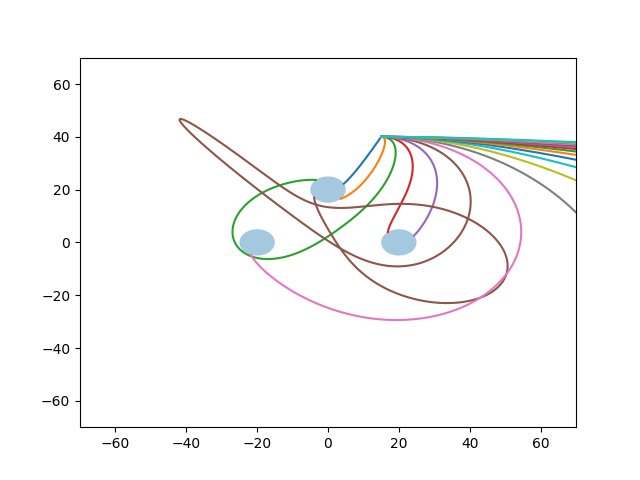
\includegraphics[width=0.5\textwidth]{desafio.png}
    \caption{Resultado}
\end{figure}

\end{document}


